% You should title the file with a .tex extension (hw1.tex, for example)
\documentclass[a4paper, 11pt]{article}

\usepackage{amsmath}
\usepackage{amssymb}
\usepackage{fancyhdr}
\usepackage{graphicx}
\usepackage{scribe}
\usepackage{tikz}
\usepackage{graphicx}
\usepackage[margin=1in]{geometry}
\usepackage{graphicx}
\newcommand{\question}[2] {\vspace{.25in} \hrule\vspace{0.5em}
\noindent{\bf #1: #2} \vspace{0.5em}
\hrule \vspace{.10in}}
\renewcommand{\part}[1] {\vspace{.10in} {\bf (#1)}}

\newcommand{\myname}{Kriangsak T., Hasdin G.}
\newcommand{\myemail}{kriangsak.thi@student.mahidol.edu, hasdin.g@student.mahidol.edu}
\newcommand{\myhwnum}{2.1}

\setlength{\parindent}{0pt}
\setlength{\parskip}{5pt plus 1pt}
 


\begin{document}

\medskip                        % Skip a "medium" amount of space
                                % (latex determines what medium is)
                                % Also try: \bigskip, \littleskip

\thispagestyle{plain}
\begin{center}                  % Center the following lines
{\Large ICCS240: Assignment \myhwnum} \\
\myname \\
\myemail \\
Collaborator: {1409l}
\end{center}
\section{Yelp}
\subsection{Report of Schema}
	This database has four relations:  
	\begin{itemize}
	\item \textsc{business}(\underline{businessId} char,
	name varchar,
	address varchar,
	city varchar,
	state varchar,
	postalCode varchar,
	stars float,
	isOpen numeric(1),
	reviewcount numeric)
	
	\textit{Primary Key} : businessId
	\item \textsc{user}(\underline{userId} char(22), 
	name varchar,
	 reviewCount numeric, 
	 averageStars float)
	 
	 \textit{Primary Key} : userId
	 
	 \item \textsc{eliteuser}(\underline{userIdd} char(22), elite INTEGER)
	 
	 \textit{Foriegn key}: userId
	 
	 \textit{Reference} : \textsc{users}(userId)
	 
	\item \textsc{review}(\underline{reviewId} char(22),
\underline{userId} char(22),
\underline{businessId} char(22),
stars integer,
 useful integer,
text varchar,
year integer) 

	 \textit{Primary key}: reviewId
	 
	  \textit{Foriegn key}: userId, businessId
	  
	\end{itemize}
	
		Where \textsc{business} has customers known as \textsc{user} where some users can be categorized as \textsc{elite} status by any business if certain requirements are met. Also, each of the users can review any business service used.
\subsection{Indexes}
The following indexes are created as means of efficient queries. We chose to hash the attributes whose likelihood in being queried upon is relatively high. 
\begin{verbatim}
create  index business1 on business using hash(business_id);
create  index business2 on business using hash(address);
create  index business3 on business using hash(city);
create  index business4 on business using hash(stars);
create  index business5 on business using hash(review_count);
create  index business6 on business using hash(is_open);
create  index business7 on business using hash(state);
create  index business8 on business using hash(name);
create  index users1 on users using hash(user_id);
create  index users2 on users using hash(name);
create  index users3 on users using hash(average_stars);
create  index users_elite1 on elite_users using hash(elite);
create  index review1 on review using hash(user_id);
create  index review2 on review using hash(stars);
create  index review3 on review using hash(text);
create  index review4 on review using hash(business_id);
create  index review5 on review using hash(year);
\end{verbatim}

\subsection{Queries}
		\begin{itemize}
		\item[(1)] Still In Business:
		\begin{verbatim}
		SELECT business_id,CONCAT(address,city,state,postal_code) AS   	
		full_address, stars  FROM business  WHERE is_open =1 AND state = state 
		ORDER BY review_count DESC LIMIT 10;
		\end{verbatim}
		\item[(2)] Top Reviews
		\begin{verbatim}
		SELECT u.user_id, u.name, review.stars, business_id FROM review 
		INNER JOIN users u ON business_id= input 
		ORDER BY review.useful DESC  LIMIT 5;
		\end{verbatim}
		\item[(3)] Average Rating
		\begin{verbatim}
		SELECT user_id, name AS name_of_user, average_stars AS 
		average_star_ratings WHERE user_id = id_input;
		\end{verbatim}
		\item[(4)] Top Business in City
		\begin{verbatim}
SELECT a.business_id, b.name, b.review_count, stars, countt
FROM (SELECT cit.business_id, COUNT(*) countt
FROM (SELECT business_id, review.user_id
FROM review
   INNER JOIN elite_users answer
   ON answer.user_id = review.user_id AND answer.elite = review.year) el
   INNER JOIN (SELECT * FROM business
   WHERE city = InputCity) cit
   ON cit.business_id = el.business_id
   GROUP BY cit.business_id
   HAVING COUNT(*) > InputeliteCount
   ORDER BY COUNT(*) DESC LIMIT InputTopCount) a
   INNER JOIN (SELECT * FROM business WHERE city = InputCity) b 
   ON b.business_id = a.business_id;
		\end{verbatim}
		\end{itemize}
\subsection{Performance Bench-marking}
From our experimental results, without indexing, some queries will take a few seconds to output, with indexing, we can run queries within milliseconds. The detailed numerical result is as follows:
For 
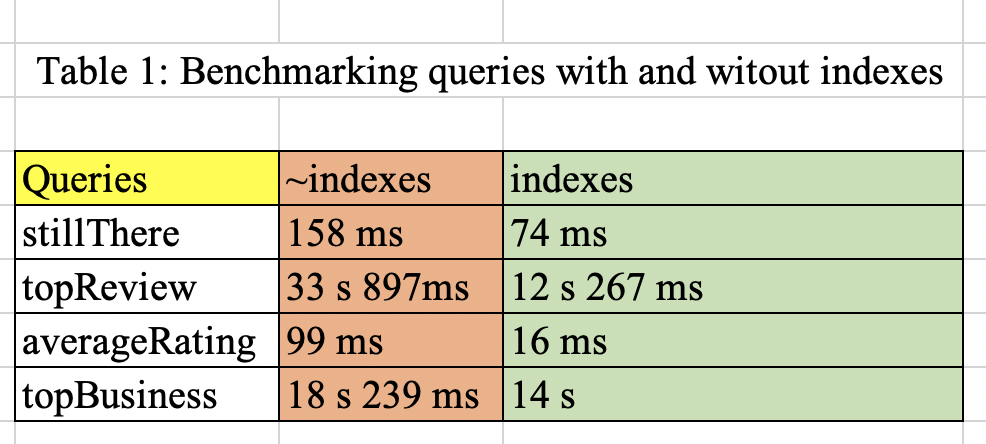
\includegraphics[width=\textwidth]{thisisreal.png}

Of note, noticed that the first query run after indexing did not perform much better due to heavy-seek searches. 

\end{document}

